\documentclass{article}
\usepackage[utf8]{inputenc}
\usepackage[brazilian]{babel}
\usepackage[utf8]{inputenc}
\usepackage[T1]{fontenc}
\usepackage{amssymb}
\usepackage{url}
\usepackage{listings}
\usepackage{xcolor} 

\usepackage{graphicx}
\graphicspath{ {./} }

\newcommand*\barra[2][]{\overline{ #1_{#2} }}

\lstset{
    frame=tb, 
    tabsize=2,
    showstringspaces=false,
    numbers=left, 
    commentstyle=\color{gray}, 
    keywordstyle=\color{blue}, 
    stringstyle=\color{red} 
}

\title{Trabalho de Simulação de MAB-515}
\author{ Gabriel Bhering Dominoni }
\date{12 de Julho de 2019}

\begin{document}

\maketitle
\thispagestyle{empty}

\pagebreak

\tableofcontents

\pagebreak

\section{Introdução}
O simulador foi implementado em C++, utilizando de todos os recursos da linguagem para máxima eficiência. A constantes do programa - lambda, disciplina, kmin e outros - são definidas em código pré-compilação para que o compilador possa otimiza-las. \\

Há uma estrutura que aramazena os eventos, contentdo simplesmente o tempo para quando o evento está agendado, um indicador da rodada a qual o evento pertence e um campo para o tipo. No mesmo arquivo onde a estrutura está definida, também há um enum contendo os nomes dos tipos. Além disso, a estrutura tem um construtor trivial e implementações de comparadores relacionais para facilitar testar qual evento acontece antes. \\

Os eventos são armazenados numa fila de prioridade que ordena eventos cronologicamente. A função principal insere a primeira chegada, e roda a simulação pelo número definido de rodadas, resultando em um par de vetores com as $\barra{W}$ e $\barra{N_q}$ de cada rodada. Cada rodada termina quando kmin coletas de tempo de espera acontecem, equivalente a kmin entradas no servidor. Ao fim das rodadas as variancias e médias entre rodadas são então calculadas. \\

Há apenas dois tipos de evento nesta simulação: chegads e partidas. Quando qualquer evento é tratado, estatisticas referentes ao número de pessoas em espera, calculando incrementamente a área do grafico pessoas em espera x tempo. Chegadas aumentam o número de pessoas na fila, e o número de pessoas em espera quando há um serviço ocorrendo, além de agendar uma partida caso não haja outros fregueses na fila. Partidas naturamente diminuem os contadores de fila e espera (se necessário) além de agendar a próxima partida caso haja pelo menos um fregues em espera. \\

As chegadas que não são processadas imediatamente são armazenadas em uma lista, equivalente a simulação explícita da fila de espera. Quando uma partida ocorre, se houver alguém em espera, um novo evento de partida é agendado e uma chegada é consumida para gerar estatística referente aos tempos de espera. A espera consumida vem do fim da fila se LCFS, ou do início, se FCFS. Estatisticas referentes a espera só são computadas se a chegada em questão pertence aquela rodada. \\

Quanto a facilidades de geração de números aleatórios, a biblioteca padrão da linguagem disponibiliza diversos geradores e consumidores. Geradores são objetos que geram sequencias pseudo-aleatórias e consumidores transformam os items da sequencia em distribuições e etc. Foram utilizados os mais básicos disponiveis: o gerador padrão e o consumidor uniforme. Para a maioria dos experimentos foi utilizada a semente 51520191. Para comprovar independencia de semente, é fácil obter o estado atual do gerador e utiliza-lo para seguir a sequencia.

\section{Testes de Correção}
Os primeiro teste feito foi o caso trivial, reduzindo a simulação para D/D/1. Como esperado, para casos onde a taxa de serviço é maior do que a de chegada, todas as estatísticas retornaram zero. Quando o serviço é menor, a fila cresceu exponencialmente.

Após, testes onde a capacidade do programa de gerar novas chegadas foi suprimida e em cada rodada foi colocada uma distribuição deterministica de fregueses. Foram feitos os seguintes testes com os seguintes resultados, cada qual com 3200 rodadas:

\begin{itemize}
\item KMIN chegadas simultaneas em T \\
E[W]=4592.51 E[Nq]=5000.49 Var[W]=106925 Var[Nq]=1314.99 
\item KMIN chegadas começando em T com 1 segundo de diferença \\
E[W]=16.4833 E[Nq]=16.3933 Var[W]=416.089 Var[Nq]=405.889 
\end{itemize}



\section{Estimativa da fase transiente}
Para estimar a fase transiente, o programa foi ligeriamente modificado. Um terceiro tipo de evento foi adicionado: deltat. Tudo que acontece quando um evento deltat é processado é coletar uma diferença entre o número de pessoas no último deltat e  agendar um novo. Podemos observar a diferença entre números de pessoas para estimar estabilidade. Os resultados foram um tanto complicados de interpretar.

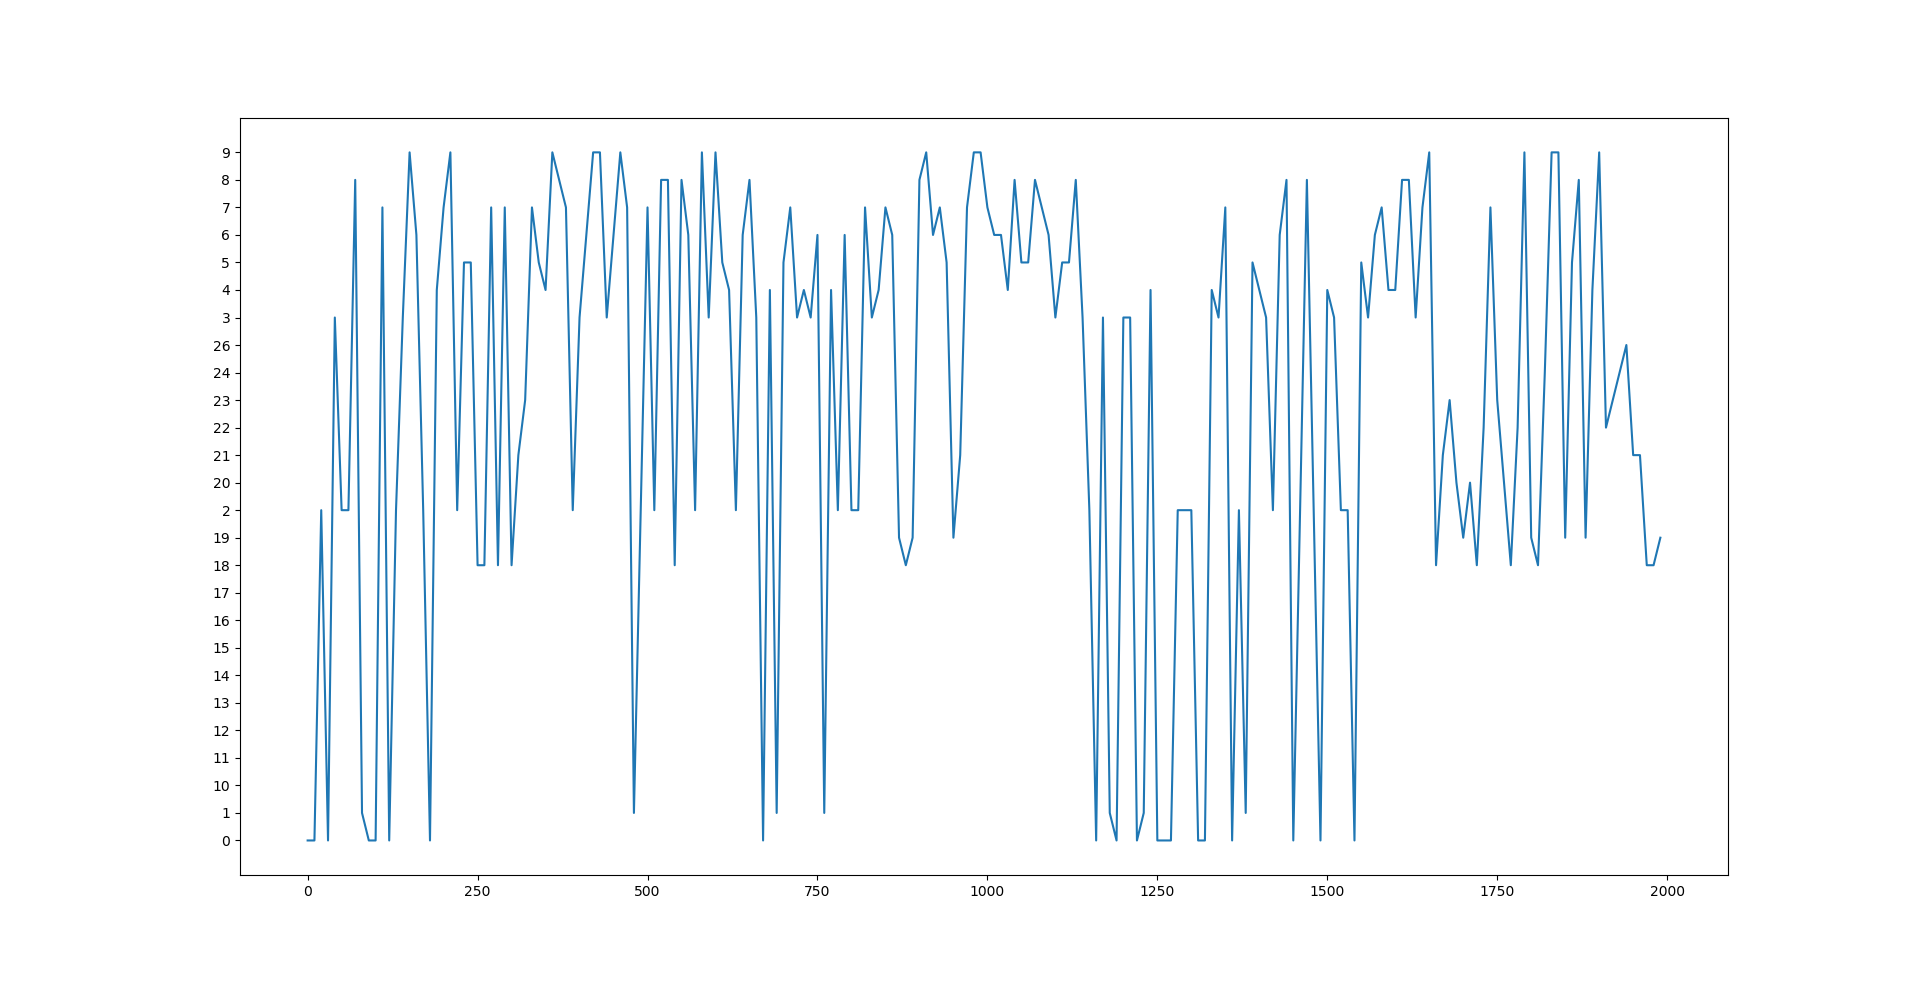
\includegraphics[width=\textwidth]{n_evo_1.png}

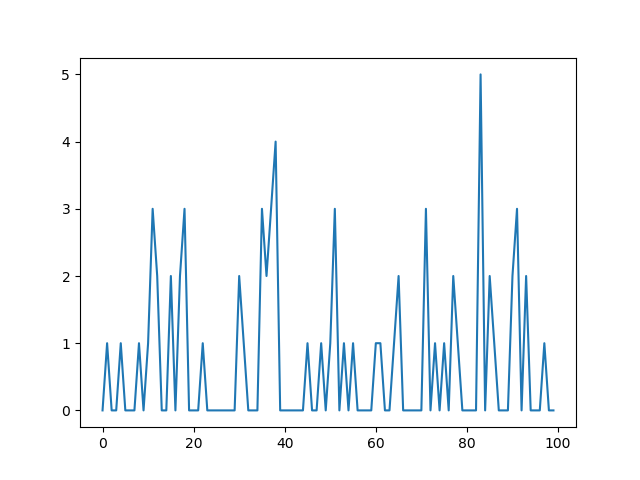
\includegraphics[width=\textwidth]{n_evo_2.png}

Na primeira figura, observamos o número de pessoas no sistema ao longo de 2000 segundos com taxa 0.9. Na segunda ao longo de 100, com taxa 0.4. Não é trivial observar onde começa a fase transiente. As coletas de deltat não ajudaram muito, tendo variações bruscas ao longo do experimento sem aparentemente estabilizar.

\section{Resultados}
\subsection{Resultados da Simulação}
Utilizando k = 2000, e 3200 rodadas.
\begin{center}
\begin{tabular}{||c c c c c c||} 
 \hline
  $\lambda$ & $\barra{W}$ & $Var(W_{FCFS})$ & $Var(W_{LCFS})$ & $\barra{N_q}$ & $Var(N_{q})$ \\ [0.5ex] 
 \hline
0.2 & 0.274 & 0.001188 & 0.001187 & 0.055 & 0.00005 \\
0.4 & 0.69193 & 0.006 & 0.00599 & 0.278 & 0.0011 \\
0.6 & 1.540 & 0.0485 & 0.0483 & 0.931 & 0.0209 \\
0.8 & 4.01 & 24 & 0.9809 & 3.3 & 0.7473 \\
0.9 & 9.03021 & 15.0802 & 11.2732 & 8.2334 & 13.4159 \\
 \hline
\end{tabular}
\end{center}

\subsection{Resultados Analíticos}
\begin{center}
\begin{tabular}{||c c c c c c||} 
 \hline
  $\lambda$ & $\barra{W}$ & $Var(W_{FCFS})$ & $Var(W_{LCFS})$ & $\barra{N_q}$ & $Var(N_{q})$ \\ [0.5ex] 
 \hline
0.2 & 0.25 & 0.5625 & 0.71875 & 0.05 & 0.0725 \\
0.4 & 0.66... & 1.77... & 3.259259... & 0.266... & 0.5511... \\
0.6 & 1.5 & 5.25 & 16.5 & 0.9 & 2.79 \\
0.8 & 4 & 24 & 184 & 3.2 & 18.56 \\
0.9 & 9 & 99 & 1719 & 8.1 & 88.29 \\
 \hline
\end{tabular}
\end{center}

\subsubsection{Fórmulas Analíticas}
\begin{center}
\begin{tabular}{||c c c||} 
 \hline
  & Média & Variância  \\ [0.5ex] 
 \hline
 W_{FCFS} & $\frac{\lambda}{1-\lambda}$ & $\frac{2\lambda-\lambda^2}{(1-\lambda)^2}$  \\ [2ex] 
 W_{FCFS} & $\frac{\lambda}{1-\lambda}$ & $\frac{2\lambda-\lambda^2+\lambda^3}{(1-\lambda)^3}$  \\ [2ex] 
 N_q & $\frac{\lambda^2}{1-\lambda}$ & $\frac{\lambda^2+\lambda^3-\lambda^4}{(1-\lambda)^2}$  \\ [2ex] 
 \hline
\end{tabular}
\end{center}

Conheçemos $N_q(z)$ (p. 91 apostila), conheçemos $N(z)$ e seus dois primeiros momentos (p. 90 apostila) e conheçemos $X^*$ (serviço exponencial com taxa 1). 

\[ N_q(z) = \frac{ N(z) - ( 1 - \lambda ) }{ z } \therefore N_q' (z) = \frac{N'(z)}{z} + \frac{N'(z)}{-z^2}\]

Substituindo $z=1$

\[ N_q' (1) = E[N] + N(z) - (1-\lambda)\]


\section{Conclusões}
Foi uma dificuldade muito grande entender a construção dos intervalos de confiança e fazer as derivações a partir das transformadas. Além disso, muito tempo foi perdido tentando fazer um simulador que funcionasse perfeitamente para ambas as disciplinas (FCFS e LCLS) sem necessidade de armazenar os tempos de chegada. Foram inúmeras versões até que a decisão de ter a fila de chegadas que ainda não entraram no servidor facilitou a implementação final. \\

É possível simular M/M/1 FCFS ainda mais rapidamente, apenas armazenando o momento da próxima chegada e trabalhando com o $W_0$ que cada chegada encontra. Os tempos de serviço são gerados assim que a chegada é processada, e, já que apenas desejavamos calcular espera e pessoas em espera, não há qualquer necessidade de se preocupar com ele novamente. Uma versão desta implementação em python está disponível no repositório. \\

A implementação final é eficiente e rápida, mas está limitada pelo tamanho do float na máquina. Com um milhão de coletas só é possível executar cerca de 400 rodadas antes que os tempos tendam a infinito por conta do contador de tempo estourar. Seria possivel resolver isso recuando o tempo em todas as partes do sistema ao se chegar a um limite ou implementando épocas ou eras. \\

Além disso gostaria de ter implementado mais gráficos, e implementado estimativa de fase transiente dinamica. Seria ideal ter modularizado mais o programa, para que fosse possivel criar uma lib reutilizavel.

\section{Anexo}

O código se encontra em: \url{github.com/gbhering/simulador-ad-2019}. \\

O código fonte sem as rotinas de geração de gráfico são C++ canonico, então pode ser compilado em qualquer sistema suportado. Para conveniencia, está incluso um Makefile com comandos para compilar normalmente, compilar otimizadamente e limpar a pasta.

\subsection{O Arquivo Principal}
\begin{verbatim}
// Constantes do programa
bool const FCFS = true;
unsigned const RODADAS = 200;
float const KMIN = 100;
float const MI = 1.0;
float const LAMBDA = 0.4;
unsigned const VERBOSE = 1;

float W[RODADAS] = {};
float N_q[RODADAS] = {};

// Variaveis da execução
float T = 0.0;          // Tempo do simulador
float N = 0;          // Pessoas encontradas no sistema 
unsigned R = 0;         // Contador de Rodada
priority_queue<Evento> fila;  // Nossa fila de eventos
deque<Evento> espera;     // Os tempos de chegada para medida futura

/* 
  A única dinstinção entre as duas disciplinas implementadas está aqui.
  Os tempos de chegadas na fila são em uma fila de duas pontas quando
  um evento de chegada é processado. Esta função agenda um novo evento
  de partida e consome uma chegada computada, da frente da fila se FCFS
  ou de trás se LCFS. Tempos de espera são calculados aqui. Apenas se
  a chegada consumida pertence a rodada atual.
*/
void entra_servidor(float& w_i, float& k) {
  fila.emplace(partida, T + exponencial(MI), R);
  if constexpr (FCFS) {
    Evento proximo = espera.front();
    espera.pop_front();
    k += (proximo.r == R);
    w_i += (proximo.r == R) ? T - proximo.t : 0;
  }
  else {
    Evento proximo = espera.back();
    espera.pop_back();
    k += (proximo.r == R);
    w_i += (proximo.r == R) ? T - proximo.t : 0;
  }
}

/*
  Esta função é a que executa o loop de cada rodada. Até que KMIN coletas de 
  tempos de espera sejam feitas, a rodada continua. 
*/
void rodada() {
  float k = 0, w_i = 0, N_qi = 0, t0 = T;
  while (k <= KMIN and !fila.empty()) {
    // Pirmeiro evento da fila é extraído
    Evento e = fila.top();  fila.pop();
    float delta = e.t - T;
    // Tempo avança
    T = e.t;
    // Número de pessoas é computado
    N_qi += espera.size()*delta;
    // Caso o próximo evento seja uma chegada...
    if ( e.tipo == chegada ) {
      // Uma nova pessoa entra no sistema 
      N++; 
      // Esta chegada é aramazenada
      espera.push_back(e);
      // Próxima chegada é agendada
      fila.emplace(chegada, T + exponencial(LAMBDA), R);
      // Caso seja a única pessoa no sistema, 
      if ( N == 1 ) 
        // entra imediatemente no servidor
        entra_servidor(w_i, k);
    } 
    // Caso o próximo evento seja uma partida...
    else if ( e.tipo == partida ) {
      // Uma pessoa sai do sistema
      N--;
      // Se ainda há pessoas no sistema, agenda uma nova partida
      if ( N > 0 ) 
        entra_servidor(w_i, k);
    }
  }

  // Guarda-se as estatisticas ao fim da rodada em vetores 
  // O total de tempo esperado é dividido pelo número de pessoas
  W[R] = w_i/KMIN; 
  // O resultado da área do gráfico é dividido pelo tempo total 
  N_q[R] = N_qi/(T-t0);
  if (VERBOSE > 0) 
    cout << R<< '(' << W[R] << ", " << N_q[R] << ')' << endl;
} 


int main(void) {
  // primeira chegada é agendada
  fila.emplace(chegada, T + exponencial(LAMBDA), R);
  while (R++ < RODADAS) 
    rodada();

  // ao fim das rodadas, calculamos as médias...
  float ENq = 0, VNq = 0, EW = 0, VW = 0;
  for (unsigned i = 0; i <= RODADAS; ++i) {
    ENq += N_q[i]/RODADAS;
    EW += W[i]/RODADAS;
  }
  // ...depois as variancias
  for (unsigned i = 0; i <= RODADAS; ++i) {
    VNq += pow( (N_q[i]-ENq), 2 ) / ( RODADAS-1 );
    VW += pow( W[i]-EW, 2 ) / ( RODADAS-1 );
  }
}
\end{verbatim}

\subsection{O Gerador}
\begin{verbatim}
std::default_random_engine gen(51520191);
std::uniform_real_distribution<double> uniform(0.0,1.0);

// Função para gerar intervalos exponenciais, 
// utilizando uma uniforme(0,1) e a inversa da CDF exponencial
inline float exponencial(float const _taxa) {
  return -log(1.0-uniform(gen))/_taxa;
} 
\end{verbatim}

\subsection{A Estrutura}
\begin{verbatim}
// apenas para conveniencia, os tipos tem nomes próprios
enum Tipo { chegada, partida };

// A estrutura que armazena os dados do eventos exponenciais
struct Evento {
  Tipo tipo;    // Chegada ou partida
  double t;     // Tempo quando acontece
  unsigned r;   // Identificador da rodada

  // Construtor trivial, existe para que seja possível criar novos eventos com facilidade
  Evento(Tipo tipo, double t, unsigned r) : tipo(tipo), t(t), r(r) {};
  // Comparadores entre eventos, para facilitar identificar quais acontecem antes
  bool operator<(const Evento& that) const { return this->t > that.t; };
  bool operator>(const Evento& that) const { return this->t < that.t; };
};
\end{verbatim}

\end{document}

